% Template for PLoS
% Version 3.4 January 2017
\documentclass[10pt,letterpaper]{article}
\usepackage[top=0.85in,left=2.75in,footskip=0.75in]{geometry}

% amsmath and amssymb packages, useful for mathematical formulas and symbols
\usepackage{amsmath,amssymb}

% Use adjustwidth environment to exceed column width (see example table in text)
\usepackage{changepage}

% Use Unicode characters when possible
\usepackage[utf8x]{inputenc}

% textcomp package and marvosym package for additional characters
\usepackage{textcomp,marvosym}

% cite package, to clean up citations in the main text. Do not remove.
% \usepackage{cite}

% Use nameref to cite supporting information files (see Supporting Information section for more info)
\usepackage{nameref,hyperref}

% line numbers
\usepackage[right]{lineno}

% ligatures disabled
\usepackage{microtype}
\DisableLigatures[f]{encoding = *, family = * }

% color can be used to apply background shading to table cells only
\usepackage[table]{xcolor}

% array package and thick rules for tables
\usepackage{array}

% create "+" rule type for thick vertical lines
\newcolumntype{+}{!{\vrule width 2pt}}

% create \thickcline for thick horizontal lines of variable length
\newlength\savedwidth
\newcommand\thickcline[1]{%
  \noalign{\global\savedwidth\arrayrulewidth\global\arrayrulewidth 2pt}%
  \cline{#1}%
  \noalign{\vskip\arrayrulewidth}%
  \noalign{\global\arrayrulewidth\savedwidth}%
}

% \thickhline command for thick horizontal lines that span the table
\newcommand\thickhline{\noalign{\global\savedwidth\arrayrulewidth\global\arrayrulewidth 2pt}%
\hline
\noalign{\global\arrayrulewidth\savedwidth}}


% Remove comment for double spacing
%\usepackage{setspace}
%\doublespacing

% Text layout
\raggedright
\setlength{\parindent}{0.5cm}
\textwidth 5.25in
\textheight 8.75in

% Bold the 'Figure #' in the caption and separate it from the title/caption with a period
% Captions will be left justified
\usepackage[aboveskip=1pt,labelfont=bf,labelsep=period,justification=raggedright,singlelinecheck=off]{caption}
\renewcommand{\figurename}{Fig}

% Use the PLoS provided BiBTeX style
% \bibliographystyle{plos2015}

% Remove brackets from numbering in List of References
\makeatletter
\renewcommand{\@biblabel}[1]{\quad#1.}
\makeatother

% Leave date blank
\date{}

% Header and Footer with logo
\usepackage{lastpage,fancyhdr,graphicx}
\usepackage{epstopdf}
\pagestyle{myheadings}
\pagestyle{fancy}
\fancyhf{}
\setlength{\headheight}{27.023pt}
\lhead{
\includegraphics[width=2.0in]{PLOS-submission.eps}}
\rfoot{\thepage/\pageref{LastPage}}
\renewcommand{\footrule}{\hrule height 2pt \vspace{2mm}}
\fancyheadoffset[L]{2.25in}
\fancyfootoffset[L]{2.25in}
\lfoot{\sf PLOS}

%% Include all macros below
\newcommand{\lorem}{{\bf LOREM}}
\newcommand{\ipsum}{{\bf IPSUM}}





\usepackage{forarray}
\usepackage{xstring}
\newcommand{\getIndex}[2]{
  \ForEach{,}{\IfEq{#1}{\thislevelitem}{\number\thislevelcount\ExitForEach}{}}{#2}
}

\setcounter{secnumdepth}{0}

\newcommand{\getAff}[1]{
  \getIndex{#1}{Arizona State University}
}

\providecommand{\tightlist}{%
  \setlength{\itemsep}{0pt}\setlength{\parskip}{0pt}}

\begin{document}
\vspace*{0.2in}

% Title must be 250 characters or less.
\begin{flushleft}
{\Large
\textbf\newline{Drought variability and the robustness of agricultural social networks} % Please use "sentence case" for title and headings (capitalize only the first word in a title (or heading), the first word in a subtitle (or subheading), and any proper nouns).
}
\newline
\\
Nicolas Gauthier\textsuperscript{\getAff{Arizona State University}}\textsuperscript{*}\\
\bigskip
\textbf{\getAff{Arizona State University}}School of Human Evolution and Social Change, 900 S Caddy Mall, Tempe, AZ\\
\bigskip
* Corresponding author: Nicolas.Gauthier@asu.edu\\
\end{flushleft}
% Please keep the abstract below 300 words
\section*{Abstract}
How robust were agrarian social networks to drought? Social networks
help absorb weather-related shocks by facilitating resource flows to
afflicted settlements and population flows away from them. This property
of social networks depends on the degree to which the networks can
connect topographically accessible locations that tend to experience
different weather patterns. We thus expect rainfall covariance in space
and time to interact with patterns of landscape connectivity to
structure prehistoric social networks.

% Please keep the Author Summary between 150 and 200 words
% Use first person. PLOS ONE authors please skip this step.
% Author Summary not valid for PLOS ONE submissions.
\section*{Author summary}
How robust were agrarian social networks to drought? Social networks
help absorb weather-related shocks by facilitating resource flows to
afflicted settlements and population flows away from them. This property
of social networks depends on the degree to which the networks can
connect topographically accessible locations that tend to experience
different weather patterns. We thus expect rainfall covariance in space
and time to interact with patterns of landscape connectivity to
structure prehistoric social networks.

\linenumbers

% Use "Eq" instead of "Equation" for equation citations.
\section{\texorpdfstring{knitr::purl(``this\_file.rmd'')}{knitr::purl(this\_file.rmd)}}\label{knitrpurlthis_file.rmd}

\section{somhow use this to run the suplemental bits
first}\label{somhow-use-this-to-run-the-suplemental-bits-first}

\section{Introduction}\label{introduction}

This is why a solid intro is \emph{so} important for academic articles.
And why I recommend a 3-paragraph model: 1. why this study is needed
(preview background) 2. what this study does/finds (preview
methods/findings) 3. what this study contributes (preview discussion)

In times of drought and famine, farmers in dryland environments turn to
their social networks to avoid starvation. Food transfers among farmers
link the food supplies of distant settlements. Similarly, atmospheric
transport of moisture via local evapotranspiration and re-precipitation
can sync crop yields across distant agroecosystems. Tracing the flows of
food, water, and energy within these complex social-ecological systems
is essential for understanding their long-term behavior, and leveraging
our archaeological understanding of why societies succeed or fail will
be critical to anticipating the impact of impending climate changes on
farming communities in the developing world.

I propose to build models -- statistical, computational, and
mathematical -- of food exchange in semiarid environments, and apply
these models to an empirical archaeological case study from the
pre-Hispanic American Southwest. Rates of site preservation and recovery
are exceptionally high in this region. Nearly two centuries of survey
and excavation have yielded extensive, high quality settlement pattern
data.

Late pre-Hispanic US Southwest -- Detailed inventories of material
culture at nearly 1,000 archaeological sites provide an unparalleled
view of the structure and dynamics of past social networks, and the
climate of this period has been intensively studied by
paleoclimatologists and climate modelers. Here, I will use statistical
models to isolate robust social and environmental \emph{patterns} at the
macro-scale.

By combining first-principles modeling with extensive empirical
datasets, the proposed research is of a kind sorely needed in the
ongoing study of sustainability in social-ecological systems. This
interdisciplinary modeling framework, and the insights generated with
it, will be of use not only to archaeologists, but also to
anthropologists, development economists, and the broader climate-change
impact-assessment community by making tractable problems with hidden,
non-trivial human-environmental linkages.

We explore the dynamics of social networks as scoial infrastructure, a
set social relaitonhsips for redistributing food, people, and
information that increases the robustness of human populations to
environmental variability.

Alternatively, we can think of patterns of interannual variability.
After holding mean climate constant, we look at the pattern of
excursions from that mean value for each region. So it doesn't matter if
you are comparing a wet and dry location, what's important is whether
each location is wetter or dryer \emph{than average for that location}
at similar times. The benefits of interacting with populations
experiencing preidctably distnct drought patterns are obios. Social
networks allow for the flow of information between spatially distinct
popuylations, allowing agents to monitor conditions in other places,
allowing them to target locations for trade or migration.

In general, we expect climate variability to impact population tynamics
on a faster time scale than mean climate, as the latter case invovles
slower scale changes in resoruce dynamics.

The benefits of social intearctio in this context include information,
resources and trade, food excahnge, migration, marriage. Costs include
metabolic costs, social costs of moving through unfriendly territory,
water, time and related opportunity costs, difficulty of monitoring
cooperation and sanctioing freeriders, and imperfect informaiton about
where best to go. cite rautmann for idea that actual volumeof food is
less imporant that information.

benefits of maintaining social relationships

\section{Background}\label{background}

Food transfers appear to be a cultural universal
{[}{\textbf{???}},Hill2011Co-ResidenceStructure{]}, yet two distinct
strands of research divide anthropological thinking on food-exchange
systems. Evolutionary anthropologists, drawing on the behavioral ecology
literature, focus on food-sharing behaviors in terms of the evolution of
cooperation in small-scale foraging societies, with a general focus on
meat sharing on daily time scales {[}{\textbf{???}},Ziker2005,
Hames2007, Allen-Arave2008{]}. Archaeologists drawing from the economics
literature focus more on the risk-minimizing aspects of food exchange,
with a general focus on the transfer of cereals between agriculturalists
on annual to decadal time scales
{[}{\textbf{???}},Garnsey1989,Rautman1993a,Hegmon1996{]}.

These are arbitrary disciplinary distinctions. Humans transfer food on a
variety of scales and social contexts. Large-scale risk-managing food
transfers among agricultural societies are subject to the same kinds of
social dilemmas as arise from cooperative behavior in small scale
societies, and food-sharing systems minimize subsistence risk regardless
of whether risk minimization is why they originally evolved. These two
research domains require a unified theoretical approach.

Recent theoretical and empirical work has begun to address how spatial,
social, and environmental factors structure food-exchange networks
{[}{\textbf{???}},Koster2014,Hao2015,Schnegg2015{]}. Food-exchange
systems are not independent of the environment, and the biophysical
context of exchange is an important component often ignored in the
anthropological literature. A more general approach to these systems
views them as a form of social infrastructure, channeling the flow of
energy between spatially structured populations in much the same way as
food webs channel energy in ecosystems {[}1{]}.

\subsection{Food exchange, social networks, and
infrastructure}\label{food-exchange-social-networks-and-infrastructure}

Infrastructure is the filter through which humans interact with their
environment {[}2{]}. A farmer, for example, does not interact with
rainwater directly but instead uses systems of canals and fields in
coordination with a network of other farmers to manage flows of water in
space and time {[}3{]}. Canals, roads, and other forms of physical
infrastructure enable physical flows like water and people. Social
infrastructure channels information, and provides affordances for
additional mass and energy flows {[}2{]}. At their core, food-exchange
networks are clusters of social relationships that redistribute food and
people among a structured population of agents. These relationships are
a form of public, social infrastructure because they enable the transfer
of energy (calories) between populations of potentially distant resource
systems (agricultural settlements and their hinterlands). Social
networks are both intangible and irregularly mobilized, requiring
significant investment to maintain and monitor. As is the case with
physical infrastructure, social networks will degrade over time if not
actively maintained.

Social infrastructure interacts directly with physical infrastructure
because social networks often must map onto spatial networks. Metabolic
costs, such as the energy expended producing and transporting food over
space, provide constraints on energy flows in exchange systems {[}4{]}.
In any particular case, the balance between these costs and the
metabolic benefits of food transfers influences whether food is moved in
bulk to the population in need, or whether that population moves itself
to the available food. The topology of spatial networks also constrains
who can interact with whom, introducing bottlenecks and other structural
flow constraints {[}{\textbf{???}}{]}. Improvements to transportation
infrastructure, such as roads and trails, decrease the effective
distance between different settlements; failure to maintain these
transportation networks increases the effective distance
{[}{\textbf{???}}{]}.

A canal system cannot be understood in isolation from local weather and
topography, and neither can an exchange system. An idealized
food-transfer network (i.e., lacking physical or social constraints)
acts as a spatiotemporal \textbf{low-pass filter} on environmental
noise, meaning that farmers in the network receive the space-time
average crop yields given variable rainfall {[}{\textbf{???}}{]}. An
understanding of the patterns of variability in rainfall, in particular
how rainfall covaries across different nodes in the network, will thus
provide a insight into the kinds of environmental pressures that drive
food-transfer systems {[}5{]}. The \textbf{social-ecological network}
concept is useful tool for understanding how social networks fit into a
such a broader ecological system.

\subsection{The Archaeology of Social Interaction in the American
Sotuhwest}\label{the-archaeology-of-social-interaction-in-the-american-sotuhwest}

Archaeology -- because of its focus on the material correlates of human
behavior over long time spans -- is uniquely suited to address how
social and physical infrastructure modulates human interactions with the
environment. Not only do archaeologists catalogue the remains of field
systems, road networks, canals, and other components of hard
infrastructure directly, but also the ceramics, raw materials, and
luxury goods that are the material correlates of networks of exchange
and interaction.

An central principle in archaeology is that we can use the spatial and
temporal patterns of environemntal variability to predict ideal cultural
responses, and then compare those expected patterns to observed ones to
test the importance of that particular pattern of environmental
variability. {[}{\textbf{???}}{]}. This process gives archaeolgically
testable empricial implications -- that people will interact with people
who have a different risk profile. The physcal environment defines the
costs and benefits of social interaction, and provides the structuring
context in which human decision making occurs.

This is a common qualitative observation in many anthropolgical and
archaeological stuides of traditional societies (scudder1962, cashdan
2001, waddel 1975, colson 1979, speilmann 1982, 1986, cashdan 1985,
wiessner 1982, werner 1983, yengoyan 1972, duff 1998, 2002, cameron
1995, jaskoff and adams 1977, crumly 1979). There have been fewer
qualitiative tests of these patterns in anthropology (with some notable
exceptions (Strawhacker, cordell, rautman, johnson)). This study seeks
to extend the findings from these specific works to the greater
Southwest region, using a much richer colleciton of social and
evironemtal data and theory informed by complex systems.

Cordell et all investigated theimpact of preciptaion variability on
ceramic exchange in tenth-thirteenth century mesa verde. They highlight
a bimodal precipitation regime, extracted from a PC analysis of 28 tree
ring cronologies form 689-1988. They show the leading modes of
variability follow an east-west split, with a bimodal precipiation
regime in the west dominated by pacific ocean, and unimodal rpecipation
in the east dominated by cyclonic rainfall form the gulf of mexico. The
line of demarcation between regions demoniatd by each mode of
variability is a \textasciitilde{}100km wide line that varies with the
jet stream. The argue that this pattern breaks doesn ca 1239-1488, and
explain it as the source of disruption in this period as the social
networks that developed to cross it over the centuries were not able to
adapt in time to the temproariliy distinct precipitaiton regime. They
suggest that broad ceramic regions examined by archaelogists reflect
``maximal risk sharing networks.'' --how's what im doing differnt --
braoder climatedata, much more robust spatial sampling, much more
etensive quantitiative

Rautmann focused on central new mexico, 900 - 1259. Using BR similarity
coefficient and local weather station preicpitation data, she found
networks up to 50km away. This is consistent with greater inetation
within 80km due to spacing required to maintian viable breeding
population she says. She highlights differential``investment of social
nergy in the maintainance of social ties between the two areas''

Social networks are surivval networks uses the same dataset here, but
different because \ldots{}. They note that both Zuni and Hopu survive
drought

Maize to chaco \ldots{} uh just cite i guess

This problem has been the focus of many computaitonal simulations. risk
sharing works in pooling network for need based transfers(hao et al
2015) but a key factor was how well eveyrone knoew everyonelses wealth.
this is acost od distance, further away you are the les you can monitor
others for free riding janssen pop aggregation shoes climate variaiblity
impacts short term aggregation, resource dynamics long term population
levels, exchange cricial for maintianin populatiopn levels, sharing
leads to short term stability but long term degredation

hegmon - resricted sharing?

crobtree -- importance of asymmetry of debt and obligations -- from this
perspective eof's are optimal because you are most garuanteed to minimze
the asymmetry of your dbts

anderies and hegmon -- infomraiton contstaints important for migration,
need to know that your potential migration desitnation is actually a
good place to go, because if you go and you were wrong (its jsut as bad)
then thats a big costs. errors in information, such as over distance,
make people more likely to move when its actually a bad aidea and fwer
to move when its a really good idea

anderies nelseon and freeman - exchagne resources with different trisk
profiels -- even in wet environments, an dincrease in interannual
variabiliytwill decrease the robustenss of specialist food supply in
variaiotoin to rainfall -- so ag economy based on specialization is more
limited by interannual deviations than mean amount

--TODO do i need to discuss past least cost path papers in the
southwest? probably.

\subsubsection{Spatial interaction models and social
gravity}\label{spatial-interaction-models-and-social-gravity}

chester king, 1976, 289-290 is source of idea that ``the greater the
difference between thet wo resource areas, the greater the insenisty of
economic interaction and the greater the hnumber of socail bonds,
including marriages''

Johnson actually fits a gravity model to chumash marriage data The use
or gravity style statistical models is uncommon in archaeology, with
exceptions (johsnon, others he cites). The method is becoming popular in
archaeology from a dynamical perspective, but not yet from a statistical
perspective. He finds some evidence for increased marriages between
different average climate zones (coastal and inland) but the effect is
weak compared to distance and size

Tobler cappadocian speculation uses it too

To our knowledge this study is the first of its kind to use social
gravity models on archy data from statistical perspective

Here, I use two empirical archaeological case studies to explore
interactions between food exchange and ecohydrology: the late
pre-Hispanic American Southwest and the Roman Imperial period in North
Africa. These regions both span areas of about 460,000 square kilometers
centered on latitude 35°N, the rough limit of the subtropical ridge that
determines the northern extent of the world's hot deserts (Figure
\ref{fig:case-studies}). Winter rainfall is delivered by large-scale
precipitation and mesoscale storms brought by westerly winds, and summer
precipitation falls from convective storms associated with southerly
Monsoonal winds. Rainfall in both seasons varies markedly year-to-year
and, because the majority of annual precipitation can fall in only a
handful of storms, it is highly unpredictable in space. Multidecadal
drought conditions are common in these regions. Global atmospheric
teleconnections often initiate drought conditions -- unusually cool
Pacific sea surface temperatures (La Ni\textasciitilde{}\{n\}a phase of
the El Ni\textasciitilde{}\{n\}o-Southern Oscillation) in the American
Southwest. Interactions between the land and atmosphere are also strong
{[}{\textbf{???}}{]}, so the length of these dry spells often reflects
more localized positive feedbacks between vegetation and soil moisture
{[}{\textbf{???}}{]}. Vegetation growth in semiarid environments is
water limited, but vegetation itself is often a major source of this
water because of terrestrial moisture recycling. Humans in these regions
not only depend on these feedback loops -- soil moisture constrains
cereal agriculture as much as natural vegetation -- but also play an
active role in them through deforestation and irrigation.

Human populations in these environments have developed similar suites of
social and physical infrastructure to manage environmental risk. Food
storage is one effective strategy for preserving bulk grains in dry
environments, and storage features are a common archaeological find
{[}{\textbf{???}}{]}. Irrigation, in particular via runoff harvesting
infrastructure near seasonally flooded streams
(\textbf{wadis}/\textbf{arroyos}), redistributes soil moisture in space
and time to create microenvironments for agriculture. But these systems
are vulnerable to flooding and would have demanded significant labor
investments to monitor and maintain {[}{\textbf{???}},
Dominguez2005,Beckers2013AncientAsia{]}. Such strategies would have been
effective for managing small-scale variability (year-to-year and
field-to-field), but would have been vulnerable to a long-lasting,
spatially extensive droughts {[}{\textbf{???}}{]}. During such extreme
weather events, inhabitants of these regions must mobilize social
networks to -- depending on the scale and severity of the event -- move
food to afflicted settlements or move people away from them. The precise
nature of these social networks, and the means by which this social
infrastructure was provisioned, varies substantially between the case
studies.

The populations of the late pre-Hispanic period in the American
Southwest subsisted mainly on maize production, supplemented by a mix of
beans and wild proteins. Food transfers are thought to have occurred
primarily in the context of informal sharing within kin groups,
reciprocal exchange at ritual ceremonies and festivals, and residential
mobility on the scale of one to three generations {[}6{]}. The
archaeological record attests to extensive exchange networks of durable
goods such as ceramics and obsidian {[}7{]}, and there is direct (if
limited) evidence for the long-distance transport of maize
{[}{\textbf{???}},Benson2010WhoDrought{]}.

Shared regional styles of elaborate ceramic tableware suggest a major
role for commensality in cultivating relationships of solidarity, both
within and between settlements (e.g., Tomkins, 2007; Urem-Kotsou and
Kotsakis, 2007). -- talk about this in the context of ceramic similarity
-- tablewares important because they speek to ocmmensalism and feastin

\section{Results}\label{results}

\subsection{Distance Decay of Social
Interaction}\label{distance-decay-of-social-interaction}

Look at distance cutoffs, are they consistent with the figures of
50km-80km from rautman and drennen and others? johnson finds no
marriages past 60km, maize to chaco papers also have distance figure of
80km

``plateu effect'' or distance within which distance doesn't matter, from
johnson but cites olsson 1965 and crumley 1979. also cite ariadne
distance deterrence function for similar idea \textasciitilde{}5km
should be the ticket if marchetti's constant holds

\subsection{Modes of Drought and Pluvial
Variability}\label{modes-of-drought-and-pluvial-variability}

The goal here is to extract ROBUST patterns of climate variability,
moving beyond the small-scale point based year to year correlations. The
latter can easily be dominated by noise or other issues with sampling
variability. The method we use here yields similar results in
appearance, but in a more objective fashion designed specifically to
skillfully extact signalfrom noise. Note that we refer to the full range
of moisture/ aridity variability here as drought for concreteness and
simplicity.The central idea here is that drought and pluvials

\begin{figure}
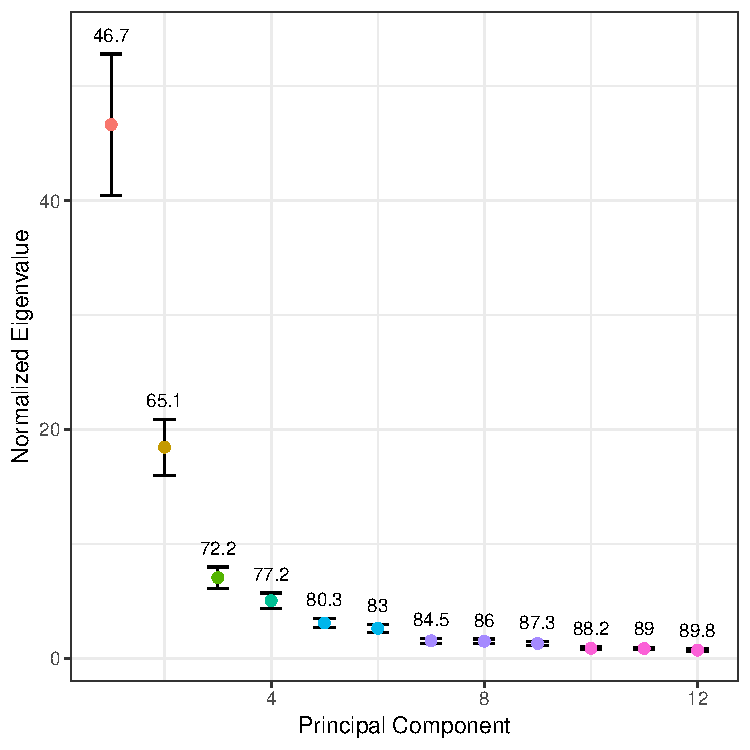
\includegraphics[width=1\linewidth]{../figures/variance_explained} \caption{Variances}\label{fig:unnamed-chunk-1}
\end{figure}

The visible drought patterns are largely consistent with those from
other studies using varied observational data and time windows. The
leading three eofs, which together explain percent of the variance
represent the influence of Pacific sea surface temperatures, and
associated anomalies such as El Nino Southern Oscillation and the
Pacific Decadal Oscillation. The fourth and fifth empriicial orthogonal
functions represent internal atmospheric variability, associated with
regional circulation patterns not influenced by the pacific. spatially
coherent

\begin{figure}
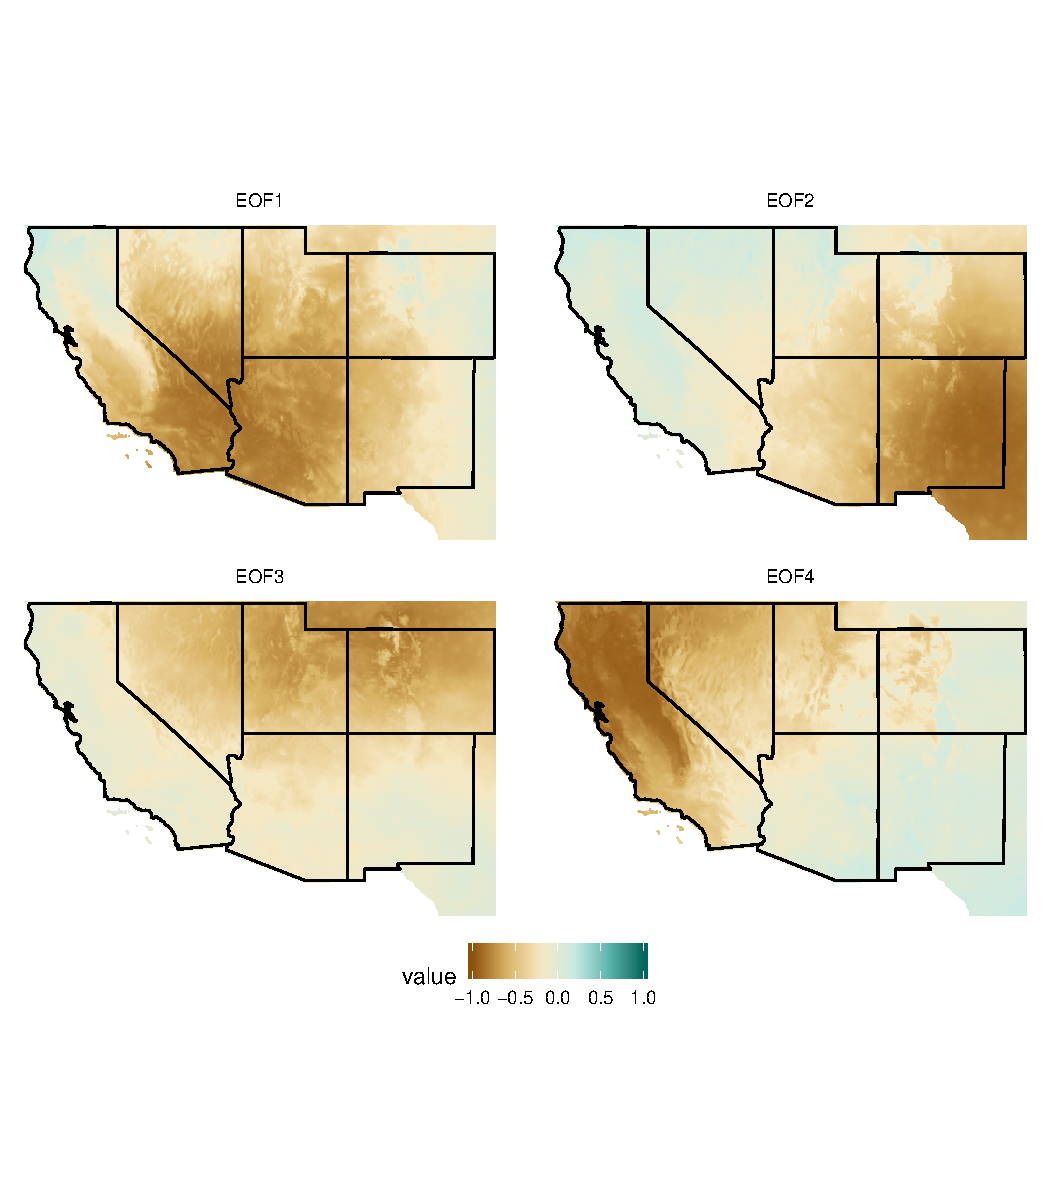
\includegraphics[width=1\linewidth]{../figures/reof_observed} \caption{Observed drought REOFs}\label{fig:unnamed-chunk-2}
\end{figure}

basic hypothesis comes down to climate patterns in terms of averages or
interannual variability. in practice, it comes down to an R-mode vs an
S-mode pca

spei is indiependend of local climatology

leading reof looks like el nino, resembles southern oscialltion pattern
(antiphase) from mccabe and dettinger 1999

distinguish between forced spatial patterns from ssts and those that are
spatilly coherent internal variability, ``noise'' in some sense, but
distinct from the spatially incoherent variability

reofs not orthogonal in spcae, but they are in time, what does that mean
for thinking about interaction?

leading 3 eigenvalues expalin nearly 70\% of the variability and reflect
ocean, consistent with mccabe et al 2004 the leading 2 specifically show
up in cook and meko resembles varimax rotate pcs from cook meko et al
1999 j climate -- summer pdsi variability

Temperature and rpecipitaiton averages are almost entirely determined by
precipitation, so we control? for that, or at least distcount it

REOF1 southwest sonoran desert zone

\subsection{Drought Variability and Social
Interaction}\label{drought-variability-and-social-interaction}

interpret relative r2 -- in johnsons chumash paper r2 was .43 for
distance and size, and adding dummy variable for same or different
enviroment only increases model to .44

do negative interactions (ie low) point to raiding and conflict?

zuni and hopi

changes in rho value over time -- pointst tomore idiosyncratic
interaction

\section{Discussion}\label{discussion}

points to disucss: 1. Why doesn't size matter? 2. Why do things change
over time? 3. What does ceramic assemblage similarity even mean? 3b.
fully connected widhgted network, but what if pruned? we argue here our
approach here is apporaprate because we are aggregating many, sparse
social networks of indivudals together at the population scale. that is
we look at macroscale flow patterns given microscale social networks,
maxent approach means we make the fest possible assumptiopns about the
configuration of the microscale social networks 5. Importance of
asymmetry. citing crabtree talk about asymmetric debts. also talk about
differences in population size and gravity model. what do we miss out on
when use symmetric data? 4. zuni and hopi? seemingly different because
different external vs internal tie patterns, but actually they both
cross climate zones 6. we just looked at summer growing season, but what
about winter (where bimodal)? Site coates et al 2015 for variability in
the seasonal phasing of rainfall 7. We don't look at the role of drought
in producing simmilarity, such as a drought leading to many migrants,
but rather look at long term patterns in the differences. This is
because we integrate out the mean of each site to get attractivities,
effectively eintegrating out utility measures (bavaud 2002, 2008). So we
are specifically looking at the ``deterrence'' effect of claimate
distances, that is the costs and beneftis of interaction.

\subsection{Qualifications, Caveats, and Future
Work}\label{qualifications-caveats-and-future-work}

jensen inequality, E(logit(y)) \textgreater{}=logit(E(y)). this means we
should interpret specific predictions and confidence intervals from this
model with caution, and instead only focus on interpretaiton of the brod
functional forms. Its a necessary evil here, becuase we do not yet have
the computational abiliy to fit the corMLPE correlation structure and a
beta family. Preliminary tests with the data suggested that the pairwise
correlation structure was a much alrger source of bias then transforming
the response variabble,so that's the tradeoffwe went with. The bias from
transforming the respone leads to bias in the estimates of variance

the eof patterns are in part scale dependent. Thihs iss isnt necesarily
a problem, its a necessity that the answer to the question what kind of
variability matters is inherently tied to the scale at which on asks the
question, there are no right or wrong answers. Although the particular
choices of variables, resolution, domain size, truncation level, were
informed here by theory and tested to as to minimze sensitivity to
paritcular choices made by the authors, different researchers could
still generate equally resonable results given different input
parameters. This is simply to state that the drought patterns
highlighted here, while we are confident they are not statistical
artifacts, should be used with caution in contexts outside of the
specific context here.

\section{Methods}\label{methods}

\subsection{Spatial interaction model}\label{spatial-interaction-model}

We start with a symmetric similarity matrix \(\mathbf{T}\) with elements
\(T_{ij} = T_{ji} = BR_{ij}\) with \(BR\) defined as the scaled
Brainerd-Robinson coefficient of similarity between the proportions of
decorated ceramic ware types.

\[BR = 1 - \sum_{k=1}^{p} \lvert P_{ik} - P_{jk} \rvert\]

where P\_\{ik\} is the proportion of ceramics of type \(k\) at site
\(i\).

This metric estimates the similarity in the ceramic discard assemplages
between pairs of sites, which in turn is a proxy for cultural
preferences, food consumption differences, access to raw materials, and
access to trade networks. The index can be loosely interpreted as a
probability of interaction between two sites, with identical patterns of
ceramic discard indicating a high likelihood of interaction via either
direct migration or trade or indirect cultural diffusion.

This is a standard metric in archaeology (cowgill 1990, golitko et al
2009, hart engelbrecht 2012), similar to the xy distances used in other
fields, and is used to .

We fit models of the form

\[T_{ij} = k v_i^\mu w_j^\alpha \exp(\beta c_{ij})\]

where \(c_{ij}\) is some notion of the generalized cost of moving from
\(i\) to \(j\) and is symmetric, meaining \(c_{ij} = c_{ji}\).

Gravity models of this form are quasisymmetric, and can be decomposed
into symmetric and asymmetric components

Which states that the flow of people, goods, or information from site
\(i\) to site \(j\) is a function of some property \(v\) of site \(i\),
property \(w\) of site \(j\), and the distance between them \(c_{ij}\)
with \(c_{ij} = c_{ji}\)

A key question is how to relate directed, asymmetric flows in \(T_{ij}\)
to the undirected, symmetric similarities in \(BR\), that is what is
\(BR = f(T_{ij},T_{ji})\), which is to say how does ceramic assemblage
similarity reflect the underlying flow of people, goods, and
information?

Question: Do regional interaction networks self-organize with respect to
patterns of climate variability, and if so at what spatial scales does
this organization occur?

Social networks help absorb weather-related shocks by facilitating
resource flows to afflicted settlements and population flows away from
them. This property of social networks depends on the degree to which
those networks can connect topographically accessible locations that
tend to experience different weather patterns. I thus expect patterns of
rainfall covariance in space and time to interact with patterns of
landscape connectivity to structure prehistoric social networks.

This relationship has been documented in the US Southwest on smaller
spatial scales, using definitions of ``climate variability'' limited by
the environmental data available in each case {[}5{]}. The proposed work
expands on these efforts to analyze the entire regional system, using
two types of climate variability derived from a paleoclimate model-data
fusion technique.

\subsection{Archaeological Social Network
Proxies}\label{archaeological-social-network-proxies}

I draw on an extensive archaeological database from the US Southwest
(Figure \ref{fig:swsn}) to address this question. The \textbf{Southwest
Social Networks} (SWSN) database is a compendium of material-culture
data from nearly 1,000 well-dated sites in Arizona and western New
Mexico from between 1200 and 1500 CE {[}8{]}. Drawing on a large sample
of sites from the earlier \textbf{Coalescent Communities} database of
all recorded prehistoric settlements with more than 12 rooms in the
Southwest from 1200 to 1700 CE {[}9{]}, the SWSN project analyzed nearly
4.7 million ceramic artifacts and nearly 5,000 obsidian artifacts
{[}10{]}. Using an index of the similarity of ceramic assemblages and
geochemical sourcing as proxies for the intensity of social interaction
between settlements, the SWSN database provides quantitative estimates
of the topology of the region-wide social network during six 50 year
time steps {[}7{]}.

\subsection{Topography and Least-Cost
Networks}\label{topography-and-least-cost-networks}

All else being equal, locations that are closer together in space will
be more similar than those further apart {[}{\textbf{???}}{]}. Modelling
this spatial structure in the SWSN data is necessary to control for
spatial dependence in statistical analyses of these data. To accomplish
this, I calculate the least-cost network between all sites in the SWSN
network. This method provides an efficient estimation of the metabolic
costs of movement between any pair of settlements in the network. I
calculate these costs using the Pandolf-Santee formula {[}11{]}, which
relates the metabolic rate of a traveler in watts to the traveler's
weight and external load, walking speed, terrain slope, and a
dimensionless terrain roughness coefficient. Using energy expenditure
rather than time or Euclidean distance to represent movement costs
facilitates a direct comparison of the metabolic costs and benefits of
food transfers {[}4{]}. The resulting least-cost network will be used as
a proxy measure for the constraints on moving both people and bulk goods
across the landscape, and thus the topographic affordances for social
exchanges.

\subsection{Paleoclimate Data
Assimilation}\label{paleoclimate-data-assimilation}

ccsm simulates monsoon ok, better than others Estimates of past
hydroclimate in the American Southwest are generated using paleoclimate
modeling tools, in particular Earth system model simulations, data
assimilation, and bias correction and spatial downscaling. Climate-model
simulations are a valuable method to estimate past, present, and future
climate states. Climate models generate physically consistent climate
fields at high temporal resolutions. These models capture the dynamic
response of the Earth's climate system to external forcing and internal
variability by resolving a series of differential equations governing
atmospheric and oceanic flow on a three-dimensional mesh of points
{[}12{]}. Recent state-of-the-art \textbf{Earth system models} extend
this approach by simulating the interactions between the atmosphere,
ocean, ice, land, and biosphere, including an array of biogeohphysical
and biogeochemical processes such as the precipitation-vegetation
feedbacks generating long-term droughts {[}13{]}.

Data assimilation techniques such as the ensemble Kalman filter are used
to generate atmospheric \textit{reanalyses}. A reanalysis is a
model-based climate hindcast optimally constrained by instrumental
observations. Paleoclimate data assimilation relies on the same
principle but replaces instrumental observations with paleoclimate proxy
records such as tree rings, ice cores, and corals {[}{\textbf{???}}{]}.
Paleoclimate model simulations serve as physically consistent prior
information about the possible states of the climate system, and the
proxy records provide novel information about the time evolution of
those states. The ensemble Kalman filter uses this information, as well
as the spatial covariances from the climate-model prior
(e.g.~teleconnections), to ``spread out'' information from the
point-based proxies to generate physically optimal extrapolations beyond
the proxy locations {[}{\textbf{???}},Hakim2016TheResults{]}.

For the late pre-Hispanic period of interest, I will use outputs from
the Community Earth System Model (CESM) Last Millennium Ensemble (LME)
as a model prior. LME is a paleoclimate simulation that uses CESM to
recreate the transient response of the global climate system to changes
in climate forcings (e.g.~orbit, greenhouse gasses, volcanic activity,
land-cover change) during the past 1,000 years {[}14{]}. The model was
run repeatedly from different initial conditions to assess the range of
internal model variability to fixed forcing mechanisms.

\subsection{Statistical inference}\label{statistical-inference}

To isolate meaningful patterns of variability in the paleo-reanalysis, I
use the model outputs to calculate a drought index and then decompose
the nearly 3,600 monthly drought maps from 1200 to 1500 CE into five
\textit{empirical orthogonal functions} (EOFs) (Figure \ref{fig:eofs}).
EOFs are the eigenvectors of the climate space-time covariance matrix,
such that the leading EOFs capture most of the variability in the
original climate signal {[}{\textbf{???}}{]}. EOFs are equivalent to the
principal component analysis commonly used in archaeology
\textbackslash{}cite{[}e.g.{]}{[}{]}\{Dean1996DemographyStress{]}, save
for that the principal components of a spatiotemporal dataset only
capture temporal signals.

varimax rotation, scaled by the square root of the corresponding
eigenvalues

I will then use nonlinear regression (generalized additive models for
beta-distributed data {[}{\textbf{???}}{]}) to determine whether the
patterns of interaction strength from the SWSN database are
significantly related to the patterns of variability captured in the
EOFs (Figure \ref{fig:eofs}). I will compare the following hypotheses:

Null Hypothesis -- Social networks are not related to climate patterns,
and the strength of interaction between any two sites is solely a
function of their relative sizes and the distance between them.
Hypothesis 1 -- Interactions between sites in opposing EOFs are
significantly stronger than would be expected by distance alone.
Hypothesis 2 -- Interactions between sites experiencing different mean
growing-season climates are significantly stronger than would be
expected by distance alone.

We fit generalized additive mixed models, and select the most
parsimonious model from all candidate models using Akaike's Information
Criterion. AIC selection between linear mixed models outperformed
several other estimating techniques in landscape genetics in simulation
studies by {[}{\textbf{???}} et al 2018{]}. We account for
nonindependence of ovserved edges that share origin or destination sites
using the maximum likelihood population effects correlation structure,
which models the co dependence of errors on shared sites. This helps
account for the nature of pairwise data, including overpowered.

Archaeological networks have several specfic features that can make
statistical inference difficult.

\section*{References}\label{references}
\addcontentsline{toc}{section}{References}

\hypertarget{refs}{}
\hypertarget{ref-Crabtree2015}{}
1. Crabtree SA. Inferring Ancestral Pueblo Social Networks from
Simulation in the Central Mesa Verde. Journal of Archaeological Method
and Theory. Springer US; 2015;22: 144--181.
doi:\href{https://doi.org/10.1007/s10816-014-9233-8}{10.1007/s10816-014-9233-8}

\hypertarget{ref-Anderies2015}{}
2. Anderies JM. Understanding the Dynamics of Sustainable
Social-Ecological Systems: Human Behavior, Institutions, and Regulatory
Feedback Networks. Bulletin of Mathematical Biology. 2015;77: 259--280.
doi:\href{https://doi.org/10.1007/s11538-014-0030-z}{10.1007/s11538-014-0030-z}

\hypertarget{ref-Yu2015}{}
3. Yu DJ, Qubbaj MR, Muneepeerakul R, Anderies JM, Aggarwal RM. Effect
of infrastructure design on commons dilemmas in social-ecological system
dynamics. Proceedings of the National Academy of Sciences. National
Academy of Sciences; 2015;112: 13207--13212.
doi:\href{https://doi.org/10.1073/pnas.1410688112}{10.1073/pnas.1410688112}

\hypertarget{ref-Drennan1984}{}
4. Drennan RD. Long-distance transport costs in pre-Hispanic
Mesoamerica. American Anthropologist. 1984;86: 105--112.

\hypertarget{ref-Rautman1993a}{}
5. Rautman AE. Resource Variability, Risk, and the Structure of Social
Networks: An Example from the Prehistoric Southwest. American Antiquity.
1993;58: 403--424.

\hypertarget{ref-Hegmon1991}{}
6. Hegmon M. The Risks of Sharing and Sharing as Risk Reduction:
Interhousehold Food Sharing in Egalitarian Societies. 1991. pp.
309--322.

\hypertarget{ref-Mills2013a}{}
7. Mills BJ, Clark JJ, Peeples M a, Haas WR, Roberts JM, Hill JB, et al.
Transformation of social networks in the late pre-Hispanic US Southwest.
Proceedings of the National Academy of Sciences of the United States of
America. 2013;110: 5785--90.
doi:\href{https://doi.org/10.1073/pnas.1219966110}{10.1073/pnas.1219966110}

\hypertarget{ref-Mills2012}{}
8. Mills BJ, Roberts Jr JM, Clark JJ, Haas Jr WR, Huntley D, Peeples MA,
et al. The Dynamics of Social Networks in the Late Prehispanic US
Southwest. Network analysis in archaeology: New approaches to regional
interaction. Oxford University Press; 2013. pp. 181--202.

\hypertarget{ref-Hill2004}{}
9. Hill JB, Clark JJ, Doelle WH, Lyons PD. Prehistoric Demography in the
Southwest: Migration, Coalescence, and Hohokam Population Decline.
American Antiquity. 2004;69: 689--716.
doi:\href{https://doi.org/10.2307/4128444}{10.2307/4128444}

\hypertarget{ref-Mills2015a}{}
10. Mills BJ, Peeples MA, Haas, Jr. WR, Borck L, Clark JJ, Roberts, Jr.
JM. Multiscalar Perspectives on Social Networks in the Late Prehispanic
Southwest. American Antiquity. 2015;80: 3--24.
doi:\href{https://doi.org/10.7183/0002-7316.79.4.3}{10.7183/0002-7316.79.4.3}

\hypertarget{ref-White2012}{}
11. White DA. Prehistoric trail networks of the western Papagueria: A
multifaceted least cost graph theory analysis. In: White DA,
Surface-Evans SL, editors. Least cost analysis of social landscapes:
Archaeological case studies. University of Utah Press; 2012. pp.
188--206.

\hypertarget{ref-Gettelman}{}
12. Gettelman A, Rood RB. Demystifying climate models: A users guide to
Earth System Models. Berlin: Springer; 2016. p. 274.
doi:\href{https://doi.org/10.1007/978-3-662-48959-8}{10.1007/978-3-662-48959-8}

\hypertarget{ref-Hurrell2013}{}
13. Hurrell JW, Holland MM, Gent PR, Ghan S, Kay JE, Kushner PJ, et al.
The community earth system model: A framework for collaborative
research. Bulletin of the American Meteorological Society. 2013;94:
1339--1360.
doi:\href{https://doi.org/10.1175/BAMS-D-12-00121.1}{10.1175/BAMS-D-12-00121.1}

\hypertarget{ref-Otto-bliesner2015}{}
14. Otto-Bliesner BL, Brady EC, Fasullo J, Jahn A, Landrum L, Stevenson
S, et al. Climate variability and change since 850 ce an ensemble
approach with the community earth system model. Bulletin of the American
Meteorological Society. 2016;97: 787--801.
doi:\href{https://doi.org/10.1175/BAMS-D-14-00233.1}{10.1175/BAMS-D-14-00233.1}

\nolinenumbers


\end{document}

